\documentclass[tikz, border=5pt]{standalone}
\usetikzlibrary{shapes.callouts,calc,arrows,decorations.pathmorphing,intersections}
\tikzset{
  level/.style   = { thick, black }, %ultra thick
  connect/.style = { dotted, black },
  connect_vert/.style = { dashed, black },
  absorbtion/.style={thick,red,->,>=stealth',shorten >=1pt},
  emission/.style={thick,blue,->,>=stealth',shorten >=1pt},
  transition/.style={thick,black,->,>=stealth',shorten >=1pt},
  transition2/.style={thick,green,->,>=stealth',shorten >=1pt},
  %notice/.style  = { draw, rectangle callout, callout relative pointer={#1} },
  %label/.style   = { text width=2cm }
  radiative/.style={absorbtion,decorate,decoration={snake,amplitude=1.5}},
  radiative2/.style={emission,decorate,decoration={snake,amplitude=1.5}},
  radiative3/.style={transition2,decorate,decoration={snake,amplitude=1.5}},
}
\begin{document}
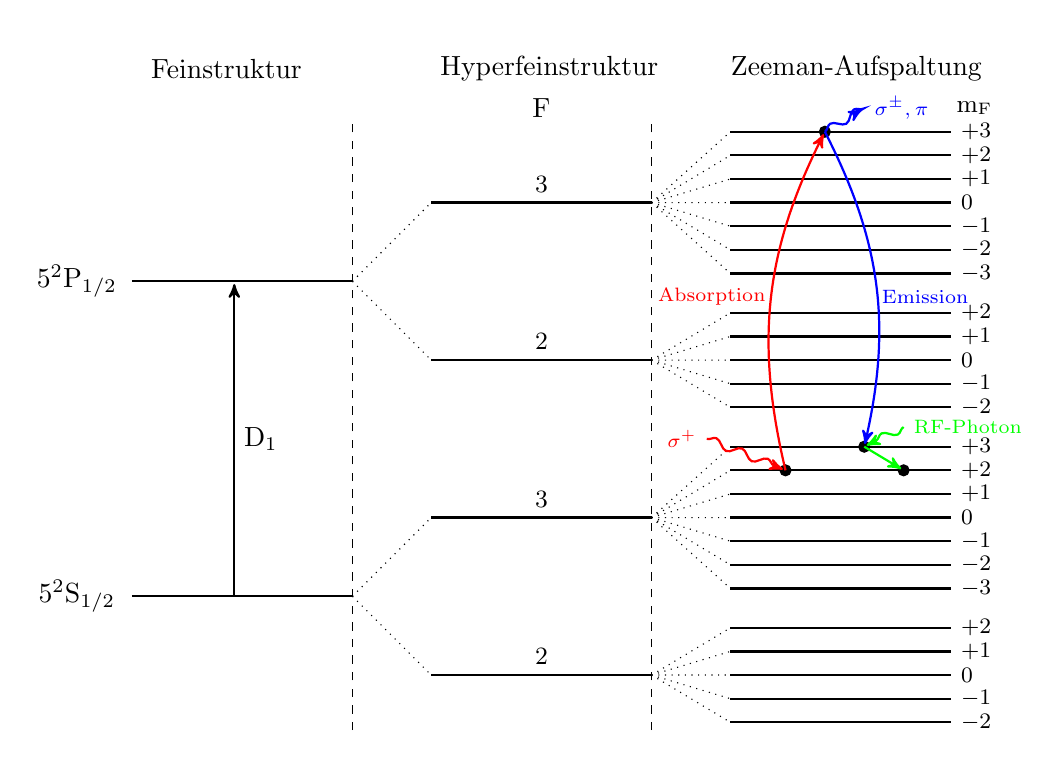
\begin{tikzpicture}
    % Draw all levels
    % Feinstrukur
    \draw[level] (0.2,1) -- (3,1);
    \draw[level] (0.2,5) -- (3,5);
  
    % Hyperfeinstruktur
    %s_1/2
    \draw[level] (4,0) -- node[above] {\small 2} (6.8,0);
    \draw[level] (4,2) -- node[above] {\small 3} (6.8,2);

    %p_1/2
    \draw[level] (4,4) -- node[above] {\small 2} (6.8,4);
    \draw[level] (4,6) -- node[above] {\small 3} (6.8,6);

    
    % Zeemanaufspaltung
    %s_1/2
    \draw[level] (7.8,-0.6) -- (10.6,-0.6) node[right] {\footnotesize $-2$};
    \draw[level] (7.8,-0.3) -- (10.6,-0.3) node[right] {\footnotesize $-1$};
    \draw[level] (7.8,0) -- (10.6,0) node[right] {\footnotesize $0$}; 
    \draw[level] (7.8,0.3) -- (10.6,0.3) node[right] {\footnotesize $+1$};
    \draw[level] (7.8,0.6) -- (10.6,0.6) node[right] {\footnotesize $+2$};

    \draw[level] (7.8,1.1) -- (10.6,1.1) node[right] {\footnotesize $-3$};
    \draw[level] (7.8,1.4) -- (10.6,1.4) node[right] {\footnotesize $-2$};
    \draw[level] (7.8,1.7) -- (10.6,1.7) node[right] {\footnotesize $-1$};
    \draw[level] (7.8,2) -- (10.6,2) node[right] {\footnotesize $0$}; 
    \draw[level] (7.8,2.3) -- (10.6,2.3) node[right] {\footnotesize $+1$};
    \draw[level] (7.8,2.6) -- (10.6,2.6) node[right] {\footnotesize $+2$};
    \draw[level] (7.8,2.9) -- (10.6,2.9) node[right] {\footnotesize $+3$};

    %p_1/2
    \draw[level] (7.8,3.4) -- (10.6,3.4) node[right] {\footnotesize $-2$};
    \draw[level] (7.8,3.7) -- (10.6,3.7) node[right] {\footnotesize $-1$};
    \draw[level] (7.8,4.0) -- (10.6,4.0) node[right] {\footnotesize $0$}; 
    \draw[level] (7.8,4.3) -- (10.6,4.3) node[right] {\footnotesize $+1$};
    \draw[level] (7.8,4.6) -- (10.6,4.6) node[right] {\footnotesize $+2$};

    \draw[level] (7.8,5.1) -- (10.6,5.1) node[right] {\footnotesize $-3$};
    \draw[level] (7.8,5.4) -- (10.6,5.4) node[right] {\footnotesize $-2$};
    \draw[level] (7.8,5.7) -- (10.6,5.7) node[right] {\footnotesize $-1$};
    \draw[level] (7.8,6) -- (10.6,6) node[right] {\footnotesize $0$}; 
    \draw[level] (7.8,6.3) -- (10.6,6.3) node[right] {\footnotesize $+1$};
    \draw[level] (7.8,6.6) -- (10.6,6.6) node[right] {\footnotesize $+2$};
    \draw[level] (7.8,6.9) -- (10.6,6.9) node[right] {\footnotesize $+3$};

    
    % connect levels
    %s_1/2
    \draw[connect] (6.8,0) -- (7.8,-0.6) (6.8,0) -- (7.8,-0.3) (6.8,0) -- (7.8,0) (6.8,0) -- (7.8,0.3) (6.8,0) -- (7.8,0.6);
    \draw[connect] (6.8,2) -- (7.8,1.1) (6.8,2) -- (7.8,1.4) (6.8,2) -- (7.8,1.7) (6.8,2) -- (7.8,2) (6.8,2) -- (7.8,2.3) (6.8,2) -- (7.8,2.6) (6.8,2) -- (7.8,2.9);
    \draw[connect] (3,1) -- (4,0) (3,1) -- (4,2);

    %p_1/2
    \draw[connect] (6.8,4) -- (7.8,3.4) (6.8,4) -- (7.8,3.7) (6.8,4) -- (7.8,4.0) (6.8,4) -- (7.8,4.3) (6.8,4) -- (7.8,4.6);
    \draw[connect] (6.8,6) -- (7.8,5.1) (6.8,6) -- (7.8,5.4) (6.8,6) -- (7.8,5.7) (6.8,6) -- (7.8,6) (6.8,6) -- (7.8,6.3) (6.8,6) -- (7.8,6.6) (6.8,6) -- (7.8,6.9);
    \draw[connect] (3,5) -- (4,4) (3,5) -- (4,6);

    

    % Draw labels
    \node[label] at (1.4,7.7)  {Feinstruktur};
    \node[label] at (5.5,7.7)  {Hyperfeinstruktur};
    \node[label] at (5.4,7.2)  {F};
    \node[label] at (9.4,7.7) {Zeeman-Aufspaltung};
    \node[label] at (10.9,7.2)  {\small m\textsubscript{F}};

    \node[label] at (-0.5,1)  {5$^2$S$_{1/2}$};
    \node[label] at (-0.5,5)  {5$^2$P$_{1/2}$};

    % vertical lines
    \draw[connect_vert] (3,-0.7) -- (3,7);
    \draw[connect_vert] (6.8,-0.7) -- (6.8,7);

    %transition
    \draw[transition] (1.5,1) -- (1.5,5);

    \node[right] at (1.5,3) {D$_1$};

    %electrons 
    \begin{scope} % Electrons
        \filldraw (8.5, 2.6) circle (.07);
        \filldraw (10, 2.6) circle (.07);
        \filldraw (9.5, 2.9) circle (.07);

        \filldraw (9.0, 6.9) circle (.07); 
        %\draw (9, 0) circle (.75);
    \end{scope}
%\draw [arrow, bend angle=45, bend left]  (8.5, 2.6) to (9.0, 6.9);
\draw[absorbtion] (8.5, 2.6) to [bend angle=20, bend left] (9.0, 6.9);
\draw[ emission] (9.0, 6.9) to [bend angle=20, bend left] (9.5, 2.9);
\draw[transition2] (9.5, 2.9) to  (10, 2.6);

\node[left,text=red] at (8.37, 4.8) {\scriptsize Absorption};
\node[right,text=blue] at (9.6, 4.8) {\scriptsize Emission};
\draw[radiative] (7.5, 3)  node[left] {\scriptsize $\sigma^+$}to (8.5, 2.6) ;
\draw[radiative2] (9.0, 6.9) to (9.5, 7.2)  node[right] {\scriptsize $\sigma^\pm,\pi$};
\draw[radiative3] (10, 3.15) node[right] {\scriptsize RF-Photon} to (9.5, 2.9)  ;

\end{tikzpicture}
\end{document}